\begin{figure}
\begin{center}
    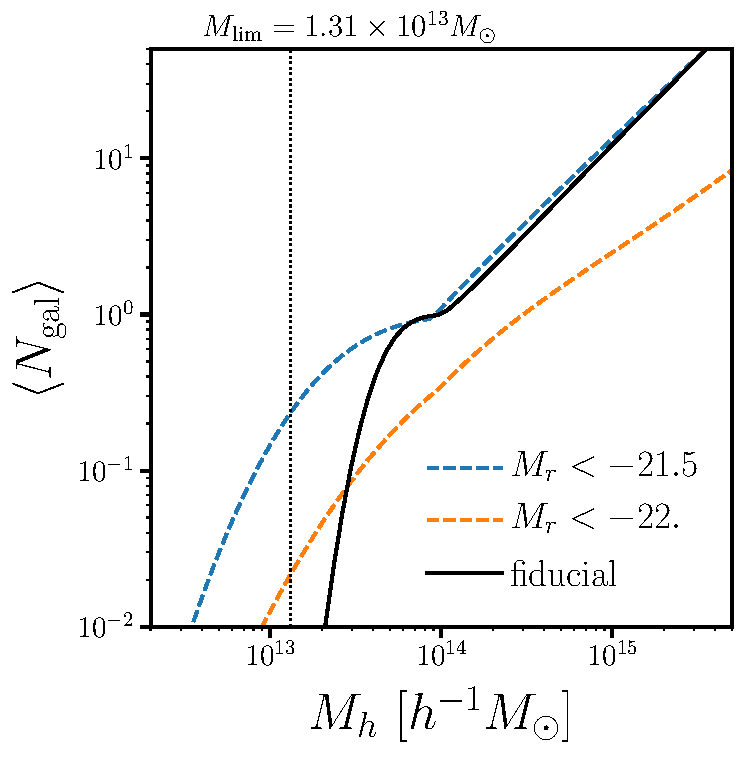
\includegraphics[width=0.45\textwidth]{figs/hod_fid.pdf} 
    \caption{
        The halo occupation our fiducial halo occupation (black) parameterized with 
        the standard \cite{zheng2007} HOD model. For the parameter values we modify
        the best-fit HOD parameters of the SDSS $M_r < -21.5$ or $< -22.$ sample
        best-fit parameters from \cite{zheng2007}. The halo mass limit of the \quij 
        simulations,  $M_{\rm lim} = 3.2\times 10^{13} h^{-1}M_\odot$ (black dashed), 
        prevent us from directly adopting the best-fit HOD parameters from \cite{zheng2007}. 
        We include the halo occupation of the \cite{zheng2007} best-fits of the 
        $M_r < -21.5$ (blue dashed) or $< -22.$ sample (orange dashed) for reference.
    }\label{fig:hod}
\end{center}
\end{figure}

\section{Halo Occupation Distribution} \label{sec:hod}  
We are interested in quantifying the information content of the galaxy bispectrum. 
For a perturbation theory approach, this involves incorporating a bias model 
for galaxies~\citep[\emph{e.g.}][]{sefusatti2006, yankelevich2019, chudaykin2019}.
Perturbation theory approaches, however, break down on small scales and limit
the constraining power from nonlinear regime. Instead, in our simulation based 
approach we use the halo occupation distribution (HOD) 
framework~\citep[\emph{e.g.}][]{zheng2005, leauthaud2012, tinker2013, zentner2016, vakili2019}.% Berlind & Weinberg 2002; Peacock & Smith 2000; Seljak 2000; Benson et al. 2000; White et al. 2001; Cooray & Sheth 2002 
HOD models statistically populate galaxies in dark matter halos by specifying
the probability of a given halo hosting a certain number of galaxies. This 
statistical prescription for connecting galaxies to halos has been remarkably 
successful in reproducing the observational statistics of galaxies (\emph{e.g.} 
galaxy clustering) and, as a result, is the standard approach for constructing 
simulated galaxy mock catalogs in galaxy clustering analyses to estimate covariance 
matrices and test systematic effects~\citep[\emph{e.g.}][]{rodriguez-torres2016, rodriguez-torres2017, beutler2017}. 
More importantly, HOD models in simulations for build galaxy clustering 
emulators~\citep[see the Aemulus project][]{mcclintock2018, zhai2018}. Emulation, 
as we mention above, is one of the most promising approaches for modeling small 
scale galaxy clustering and is what we're trying to forecast in this work. 

In the simplest HOD models, the probability of a given halo hosting $N$ galaxies 
of a certain class is dictated by its halo mass --- $P(N|M_h)$.%~\citep[\emph{e.g.}][]{zheng2007}. 
We use the standard $P(N|M_h)$ model from \cite{zheng2007}, which has been 
ubiquitously used in galaxy clustering analyses~\citep[\emph{e.g.}][\todo{many more}]{sinha2018}. 
The model specifies the mean number of galaxies in a halo as
\beq
\langle N_{\rm gal} \rangle = \langle N_{\rm cen} \rangle + \langle N_{\rm sat} \rangle
\eeq
with mean central galaxy occupation
\beq \label{eq:Ncen}
\langle N_{\rm cen} \rangle  = \frac{1}{2}\Bigg[1 + {\rm erf}\bigg(\frac{\log M_h - \log M_{\rm min}}{\sigma_{\log M}}\bigg) \Bigg]
\eeq
and mean satellite galaxy occupation
\beq \label{eq:Nsat}
\langle N_{\rm sat} \rangle = \langle N_{\rm cen} \rangle \bigg(\frac{M_h - M_0}{M_1}\bigg)^\alpha.
\eeq
The mean number of centrals in a halo transitions smoothly from 0 to 1 for halos 
with mass $M_h > M_{\rm min}$. The width of the transition is dictated by 
$\sigma_{\log M}$, which reflects the scatter between stellar mass/luminosity and 
halo mass~\citep{citecite}. For $M_h > M_{\rm min}$, 
$\langle N_{\rm sat} \rangle$ follows a power law with slope $\alpha$. $M_0$ 
is the halo mass cut-off for satellite occupation and $M_h = M_0 + M_1$ is 
the typical mass scale for halos to host one satellite galaxy. The numbers 
of centrals and satellites for each halo are drawn from Bernoulli and Poisson 
distribution, respectively. Central galaxies are placed at the center of the
halo while position and velocity of the satellite galaxies are sampled from a 
\cite{navarro1997} (NFW) profile. 

The halo occupation in the \cite{zheng2007} model depends soley on $M_h$. 
Simulations, however, find evidence that secondary halo properties such as
concentration or formation history correlate with spatial distribution of
halos --- a phenomenon referred to as ``halo assembly bias''~\citep{sheth2004, gao2005, harker2006, wechsler2006}.
A model that only depends on $M_h$, does not account for this halo assembly 
bias and may not sufficient describe the connection between galaxies and 
halos. Moreover, if unaccounted for in the HOD model, and thus not marginalized 
over, halo assembly bias may impact the cosmological parameter constraints. 
\cite{zentner2016} and \cite{vakili2019} recently examined evidence for 
assembly bias in the observed clustering measurements of the Sloan Digital 
Sky Survey (SDSS) DR 7 main galaxy sample. 
\todo{short description of the papers and how they compare with a model with assembly bias}. 
However, they find little evidence for assembly bias in the galaxy clustering
of the SDSS $M_r < -21.5$  and $-21$ samples. Therefore, in this work we use 
the standard \cite{zheng2007} HOD model and assume it is sufficient for modeling 
the galaxy--halo connection. 

For the fiducial parameter values of the HOD model we used values motivated by 
best-fit HOD parameters from the literature, namely the \cite{zheng2007} 
fits to the SDSS $M_r < -21.5$  and $-22$ samples: 
\beq \label{eq:hod_fid}
\{M_{\rm min}, \sigma_{\log M}, \log M_0, \alpha \log M_1 \} = \{13.65, 0.2, 14., 1.1, 14.\}.
\eeq
In Figure~\ref{fig:hod} we present the halo occupation of our fiducial 
HOD parameters (black). We include the best-fit halo occupations of 
the SDSS $M_r < -21.5$ (blue)  and $-22$ (orange) samples from \cite{zheng2007}
for comparison. We also mark the halo mass limit, $M_{\rm lim}$, of the \quij 
simulations (black dotted). At $M_h \sim 10^{13} M_\odot$, the best-fit halo 
occupations of the SDSS samples extend below $M_{\rm lim}$ --- \emph{i.e.} 
they have halos below $M_{\rm lim}$ that host galaxies. This prevents us from 
directly using the values from the literature and instead, we reduce 
$\sigma_{\log M}$ to 0.2 dex. We confirm using \quij simulations with higher 
mass resolution ($1024^3$ CDM particles) that $M_{\rm lim}$ does not impact
the observables or their derivatives in our analysis for our fiducial HOD 
parameters. 

As we mention above, $\sigma_{\log M}$ reflects the scatter between stellar 
mass/luminosity and halo mass. The high $\sigma_{\log M}$ in the $M_r < -21.5$ 
and $-22$ SDSS samples is caused by the turnover in this relation at high stellar 
mass/luminosity. Our fiducial halo occupation, with its lower $\sigma_{\log M}$, 
results in a galaxy sample with a tighter scatter than the samples selected based 
on $M_r$ or $M_*$ cuts, \emph{e.g.} used in SDSS and BOSS. Hence, such a sample
would require selecting based on observable galaxy properties that correlate 
more strong with $M_h$ than luminosity or $M_*$. \todo{Alpaslan et al. in prep. find
that $L_{\rm sat}$ is more correlated to $M_h$ than luminosity or $M_*$; however, 
it has yet to be used for galaxy sample selection.} Regardless, in this work
we are interested in quantifying the information content of the galaxy bispectrum 
and not analyzing an observed galaxy sample. We therefore opt for a more 
conservative set of HOD parameters with respect to $M_{\rm lim}$. 


\begin{figure}
\begin{center}
    \includegraphics[width=\textwidth]{figs/PBg_reg.pdf} 
    \caption{}
\label{fig:bgh}
\end{center}
\end{figure}


